\documentclass[
	letterpaper, % Paper size, specify a4paper (A4) or letterpaper (US letter)
	10pt, % Default font size, specify 10pt, 11pt or 12pt
]{CSUniSchoolLabReport}

%----------------------------------------------------------------------------------------
%	REPORT INFORMATION
%----------------------------------------------------------------------------------------

\title{Experiment Six\\ Fundamentals of Electromagnetics Lab \\ EECE2530/1} % Report title

\author{Michael \textsc{Brodskiy}\\ \small \href{mailto:Brodskiy.M@Northeastern.edu}{Brodskiy.M@Northeastern.edu}}

\date{November 15, 2023} % Date of the report

%----------------------------------------------------------------------------------------


\begin{document}

\maketitle % Insert the title, author and date using the information specified above

\begin{center}
	\begin{tabular}{l r}
		Date Performed: & November 8, 2023 \\ % Date the experiment was performed
        Partners: & Manas \textsc{Mahajan} \& Priyam \textsc{Modi} \\ % Partner names
		Instructor: & Professor \textsc{Marengo-Fuentes} \\ % Instructor/supervisor
        TAs: & Nicolas \textsc{Casilli} \& Farah \textsc{Ben Ayed} \\ % Teachers Assistants 
	\end{tabular}
\end{center}

\newpage

\begin{abstract}

  The goal of this laboratory experiment is to determine certain quantities, such as the ``dog-leg path differential'' and refraction index of the plexi-glass from measurements taken. A laser is pointed at the plexi-glass shape and quantities are measured in certain angles to determine these.

\end{abstract}

\begin{flushleft}

  \textsc{Keywords:} \underline{dog-leg}, \underline{refraction index}, \underline{plexi-glass}, \underline{laser}

\end{flushleft}

\newpage

\section{Equipment}

\hspace{.5 in} Available equipment included:\\

\begin{itemize}

  \item Class II Lasers with AC Power Adapter Switch

  \item Ruler

  \item Rotating Base with Tick Marks

  \item Samples to Measure Optical Properties:

    \begin{itemize}

      \item Transparent Acrylic Half-Disk

      \item Transparent Acrylic Plate

    \end{itemize}

\end{itemize}

\section{Introduction \& Objectives}

This experiment contains two parts: one in which the refraction index of the material is determined, and one in which the height difference of the dog-leg path is estimated.\\

For the refraction index measurement, we began by placing the plexi-glass shape into a slot on a rotating base. This rotating base had designated tick marks indicating various angles. A total of 17 measurements were taken, beginning from $-80^{\circ}$, and stepping in $10^{\circ}$ increments up to $80^{\circ}$.\\

For the height differential, four measurements were taken, beginning from $0^{\circ}$, and increasing in $20^{\circ}$ increments up to $60^{\circ}$. A derivation for a formula to determine the differential is then performed and used to find the value of the difference.

\section{Results \& Analysis} 

\subsection{Part I}

The table below shows our gathered data for the first part of the experiment:

\begin{center}
\begin{tabular}[H]{|c|c|}
  \hline
  $\theta_i [^{\circ}]$ & $\theta_t [^{\circ}]$\\
  \hline
  -80 & 42\\ \hline
  -70 & 39\\
  \hline
  -60 & 36\\
  \hline
  -50 & 32\\
  \hline
  -40 & 25\\
  \hline
  -30 & 20\\
  \hline
  -20 & 14\\
  \hline
  -10 & 9\\
  \hline
  0 & 2\\
  \hline
  10 & 4\\
  \hline
  20 & 11\\
  \hline
  30 & 17\\
  \hline
  40 & 22\\
  \hline
  50 & 27\\
  \hline
  60 & 32\\
  \hline
  70 & 37\\
  \hline
  80 & 41\\
  \hline
\end{tabular}
\end{center}

We can use the values in the table to estimate the index of refraction. It should be approximately the same for each incident angle. The process to find the index of refraction is applied in the example below to $80^{\circ}$:

$$n_1\sin(\theta_i)=n_2\sin(\theta_t)$$
$$n_1=1,\quad\theta_i=80,\quad\theta_t=41$$
$$n_2=\frac{\sin(80)}{\sin(41)}$$
$$n_2\approx1.472$$

This process was repeated for all values to get:

\begin{center}
\begin{tabular}[H]{|c|c|}
  \hline
  $\theta_i [^{\circ}]$ & $n_2$\\
  \hline
  -80 & 1.472\\
  \hline
  -70 & 1.493\\
  \hline
  -60 & 1.473\\
  \hline
  -50 & 1.446\\
  \hline
  -40 & 1.521\\
  \hline
  -30 & 1.462\\
  \hline
  -20 & 1.414\\
  \hline
  -10 & 1.11\\
  \hline
  0 & 0\\
  \hline
  10 & 2.489\\
  \hline
  20 & 1.792\\
  \hline
  30 & 1.71\\
  \hline
  40 & 1.716\\
  \hline
  50 & 1.687\\
  \hline
  60 & 1.634\\
  \hline
  70 & 1.561\\
  \hline
  80 & 1.501\\
  \hline
\end{tabular}
\end{center}

We should get an approximate estimate for the refraction index by taking the average of all the numbers from the table above. In doing so, we find that $n_{avg}\approx1.49\bar{8}$. Looking up the value, the expected index of refraction should be $1.4899$. Thus, our percent error is:

$$\frac{|1.49\bar{8}-1.4899|}{1.4899}\cdot100=.6029\%$$

Thus, we can see that our measurements were fairly accurate.

\subsection{Part II}

For Part II, our data was as follows:

$$t=35[\si{\milli\meter}]$$
$$0[^{\circ}]\to20[^{\circ}]=8[\si{\milli\meter}]$$
$$0[^{\circ}]\to40[^{\circ}]=13[\si{\milli\meter}]$$
$$0[^{\circ}]\to60[^{\circ}]=22[\si{\milli\meter}]$$

\begin{center}
  \begin{tabular}[H]{|c|c|}
    \hline
    $\theta_i [^{\circ}]$ & $\theta_t [^{\circ}]$\\
    \hline
    0 & 0\\
    \hline
    20 & 14\\
    \hline
    40 & 32\\
    \hline
    60 & 46\\
    \hline
  \end{tabular}
\end{center}

We begin by deriving a formula. The set up looks as follows:

\begin{figure}[H]
  \centering
  \tikzset{every picture/.style={line width=0.75pt}} %set default line width to 0.75pt        

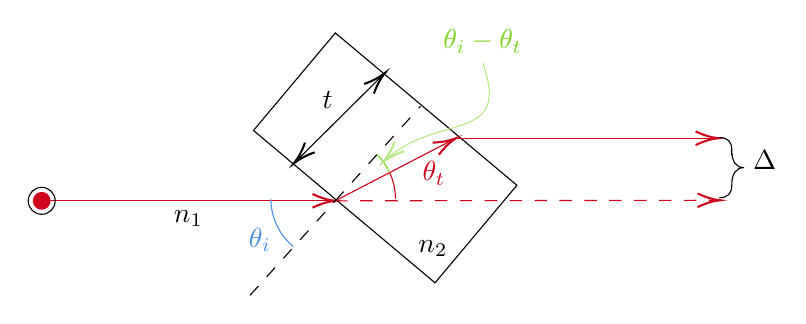
\begin{tikzpicture}[x=0.75pt,y=0.75pt,yscale=-1,xscale=1]
%uncomment if require: \path (0,444); %set diagram left start at 0, and has height of 444

%Straight Lines [id:da3089462694390681] 
\draw [color={rgb, 255:red, 208; green, 2; blue, 27 }  ,draw opacity=1 ]   (106.5,135.5) -- (245.92,135.5) ;
\draw [shift={(247.92,135.5)}, rotate = 180] [color={rgb, 255:red, 208; green, 2; blue, 27 }  ,draw opacity=1 ][line width=0.75]    (10.93,-3.29) .. controls (6.95,-1.4) and (3.31,-0.3) .. (0,0) .. controls (3.31,0.3) and (6.95,1.4) .. (10.93,3.29)   ;
%Shape: Circle [id:dp687997837864077] 
\draw   (100,135.5) .. controls (100,131.91) and (102.91,129) .. (106.5,129) .. controls (110.09,129) and (113,131.91) .. (113,135.5) .. controls (113,139.09) and (110.09,142) .. (106.5,142) .. controls (102.91,142) and (100,139.09) .. (100,135.5) -- cycle ;
%Shape: Circle [id:dp6466863455580079] 
\draw  [color={rgb, 255:red, 208; green, 2; blue, 27 }  ,draw opacity=1 ][fill={rgb, 255:red, 208; green, 2; blue, 27 }  ,fill opacity=1 ] (102.5,135.5) .. controls (102.5,133.29) and (104.29,131.5) .. (106.5,131.5) .. controls (108.71,131.5) and (110.5,133.29) .. (110.5,135.5) .. controls (110.5,137.71) and (108.71,139.5) .. (106.5,139.5) .. controls (104.29,139.5) and (102.5,137.71) .. (102.5,135.5) -- cycle ;
%Shape: Rectangle [id:dp5570623200210392] 
\draw   (247.97,54.61) -- (335.44,128) -- (296,175) -- (208.53,101.6) -- cycle ;
%Straight Lines [id:da14924518496374972] 
\draw [color={rgb, 255:red, 208; green, 2; blue, 27 }  ,draw opacity=1 ]   (247.92,135.5) -- (304.28,106.25) ;
\draw [shift={(306.05,105.33)}, rotate = 152.57] [color={rgb, 255:red, 208; green, 2; blue, 27 }  ,draw opacity=1 ][line width=0.75]    (10.93,-3.29) .. controls (6.95,-1.4) and (3.31,-0.3) .. (0,0) .. controls (3.31,0.3) and (6.95,1.4) .. (10.93,3.29)   ;
%Straight Lines [id:da36139448467369784] 
\draw [color={rgb, 255:red, 208; green, 2; blue, 27 }  ,draw opacity=1 ]   (306.05,105.33) -- (430.47,105.33) ;
\draw [shift={(432.47,105.33)}, rotate = 180] [color={rgb, 255:red, 208; green, 2; blue, 27 }  ,draw opacity=1 ][line width=0.75]    (10.93,-3.29) .. controls (6.95,-1.4) and (3.31,-0.3) .. (0,0) .. controls (3.31,0.3) and (6.95,1.4) .. (10.93,3.29)   ;
%Straight Lines [id:da36996139499499425] 
\draw [color={rgb, 255:red, 208; green, 2; blue, 27 }  ,draw opacity=1 ] [dash pattern={on 4.5pt off 4.5pt}]  (247.92,135.5) -- (431.4,135.23) ;
\draw [shift={(433.4,135.22)}, rotate = 179.91] [color={rgb, 255:red, 208; green, 2; blue, 27 }  ,draw opacity=1 ][line width=0.75]    (10.93,-3.29) .. controls (6.95,-1.4) and (3.31,-0.3) .. (0,0) .. controls (3.31,0.3) and (6.95,1.4) .. (10.93,3.29)   ;
%Shape: Brace [id:dp7371764969387753] 
\draw   (433,134) .. controls (436.98,134) and (438.97,132.01) .. (438.97,128.03) -- (438.97,128.03) .. controls (438.97,122.34) and (440.96,119.5) .. (444.94,119.5) .. controls (440.96,119.5) and (438.97,116.66) .. (438.97,110.97)(438.97,113.53) -- (438.97,110.97) .. controls (438.97,106.99) and (436.98,105) .. (433,105) ;
%Shape: Arc [id:dp6592082376861983] 
\draw  [draw opacity=0] (274.12,121.82) .. controls (275.92,125.67) and (276.92,129.97) .. (276.92,134.5) -- (246.92,134.5) -- cycle ; \draw  [color={rgb, 255:red, 208; green, 2; blue, 27 }  ,draw opacity=1 ] (274.12,121.82) .. controls (275.92,125.67) and (276.92,129.97) .. (276.92,134.5) ;  
%Straight Lines [id:da10825483880415332] 
\draw    (229.34,116.09) -- (270.56,75.21) ;
\draw [shift={(271.98,73.8)}, rotate = 135.24] [color={rgb, 255:red, 0; green, 0; blue, 0 }  ][line width=0.75]    (10.93,-3.29) .. controls (6.95,-1.4) and (3.31,-0.3) .. (0,0) .. controls (3.31,0.3) and (6.95,1.4) .. (10.93,3.29)   ;
\draw [shift={(227.92,117.5)}, rotate = 315.24] [color={rgb, 255:red, 0; green, 0; blue, 0 }  ][line width=0.75]    (10.93,-3.29) .. controls (6.95,-1.4) and (3.31,-0.3) .. (0,0) .. controls (3.31,0.3) and (6.95,1.4) .. (10.93,3.29)   ;
%Straight Lines [id:da5061477765805575] 
\draw  [dash pattern={on 4.5pt off 4.5pt}]  (247.92,135.5) -- (288.97,89.97) ;
%Shape: Arc [id:dp8090227623570767] 
\draw  [draw opacity=0] (268.13,113.29) .. controls (270.59,115.75) and (272.63,118.63) .. (274.12,121.82) -- (246.92,134.5) -- cycle ; \draw  [color={rgb, 255:red, 126; green, 211; blue, 33 }  ,draw opacity=1 ] (268.13,113.29) .. controls (270.59,115.75) and (272.63,118.63) .. (274.12,121.82) ;  
%Straight Lines [id:da6394647938540519] 
\draw  [dash pattern={on 4.5pt off 4.5pt}]  (206.87,181.03) -- (247.92,135.5) ;
%Shape: Arc [id:dp9776143180986732] 
\draw  [draw opacity=0] (227.64,157.48) .. controls (221.09,151.98) and (216.92,143.73) .. (216.92,134.5) .. controls (216.92,134.5) and (216.92,134.5) .. (216.92,134.5) -- (246.92,134.5) -- cycle ; \draw  [color={rgb, 255:red, 74; green, 144; blue, 226 }  ,draw opacity=1 ] (227.64,157.48) .. controls (221.09,151.98) and (216.92,143.73) .. (216.92,134.5) .. controls (216.92,134.5) and (216.92,134.5) .. (216.92,134.5) ;  
%Curve Lines [id:da00684858507634134] 
\draw [color={rgb, 255:red, 184; green, 233; blue, 134 }  ,draw opacity=1 ]   (319,69) .. controls (332.79,108.4) and (298.07,92.5) .. (272.16,115.71) ;
\draw [shift={(270.98,116.8)}, rotate = 316.37] [color={rgb, 255:red, 184; green, 233; blue, 134 }  ,draw opacity=1 ][line width=0.75]    (10.93,-3.29) .. controls (6.95,-1.4) and (3.31,-0.3) .. (0,0) .. controls (3.31,0.3) and (6.95,1.4) .. (10.93,3.29)   ;

% Text Node
\draw (448,116) node [anchor=west] [inner sep=0.75pt]    {$\Delta $};
% Text Node
\draw (177.21,138.9) node [anchor=north] [inner sep=0.75pt]    {$n_{1}$};
% Text Node
\draw (295,163.6) node [anchor=south] [inner sep=0.75pt]    {$n_{2}$};
% Text Node
\draw (247.95,92.25) node [anchor=south east] [inner sep=0.75pt]    {$t$};
% Text Node
\draw (218.23,147.4) node [anchor=north east] [inner sep=0.75pt]  [color={rgb, 255:red, 74; green, 144; blue, 226 }  ,opacity=1 ]  {$\theta _{i}$};
% Text Node
\draw (302.23,115.4) node [anchor=north east] [inner sep=0.75pt]  [color={rgb, 255:red, 208; green, 2; blue, 27 }  ,opacity=1 ]  {$\theta _{t}$};
% Text Node
\draw (319,65.6) node [anchor=south] [inner sep=0.75pt]  [color={rgb, 255:red, 126; green, 211; blue, 33 }  ,opacity=1 ]  {$\theta _{i} -\theta _{t}$};


\end{tikzpicture}

  \caption{Set Up for Part II}
  \label{fig:1}
\end{figure}

From the figure, we may write:

$$t=t_1\cost(\theta_t)$$

This gives us:

$$\Delta = \frac{t}{\cos(\theta_t)}\sin(\theta_i-\theta_t)$$

We may redefine the $\sin$ term as:

$$\sin(\theta_i-\theta_t)=\sin(\theta_i)\cos(\theta_t)-\sin(\theta_t)\cos(\theta_i)$$

Plugging this back into the formula for $\Delta$, we obtain:

$$\Delta=t(\sin(\theta_i)-\tan(\theta_t)\cos(\theta_i))$$

Next, we want to isolate $\theta_t$:

$$\tan(\theta_t)=\frac{\sin(\theta_i)-\frac{\Delta}{t}}{\cos(\theta_i)}$$
$$\theta_t=\tan^{-1}\left(\frac{\sin(\theta_i)-\frac{\Delta}{t}}{\cos(\theta_i)}\right)$$

Employing Snell's law, we may write:

$$n_2=\frac{n_1\sin(\theta_i)}{\sin\left( \tan^{-1} \left(\frac{\sin(\theta_i)-\frac{\Delta}{t}}{\cos(\theta_i)}\right)\right)}$$

We can use the values from the table above to calculate $n_2$. An example calculation for $\theta_i=20\left[ ^{\circ} \right]$ is shown below:

$$n_2=\frac{\sin(20)}{\sin\left(\tan^{-1}\left( \frac{\sin(20)-\frac{.008}{.035}}{\cos(20)} \right)\right)}$$
$$n_2=2.854$$

Repeating this for $\theta_i=40,60\left[ ^{\circ} \right]$, we get:

\begin{center}
  \begin{tabular}[H]{|c|c|}
    \hline
    $\theta_i\left[ ^{\circ} \right]$ & $n_2$\\
    \hline
    0 & 0\\
    \hline
    20 & 2.854\\
    \hline
    40 & 1.925\\
    \hline
    60 & 2.019\\
    \hline
  \end{tabular}
\end{center}

Once again averaging our answers, we find $n_{avg}=1.6995$, a bit less accurate than our first method, but still fairly close.

\section{Conclusion}

\subsection{Questions}

\begin{enumerate}

  \item Calculate the RI of the sample using the two methods and show the detailed optical path

    See work in the ``Results and Analysis'' section.

  \item Given the fact that the RI of plexi-glass would decrease when increasing the wavelength (optical dispersion), how would the $\theta_t$ and $\theta_r$ in the first experiment change and how would the dislocation in the second experiment change when switching the red laser to green laser?

    Given that green has a lesser wavelength than red, we know that the refraction index would increase. To compensate, the transmitted angle would have to be smaller. Since the angle would be smaller, the dislocation would be smaller as well. On the other hand, $\theta_r$ does not change, as it does not depend on the refraction index of the material being transmitted into. We know that $\theta_r=\theta_i$, and it would remain so despite any change of color.

\end{enumerate}

\subsection{Summary}

Overall, we were successfully able to use two methods to estimate the index of refraction of an acrylic/plexi-glass shape.

\end{document}
